\documentclass{umm-senior-sem}
\usepackage{cite}
\usepackage{url}

%\usepackage{setspace}
%\setstretch{2} 
\begin{document}
\conferenceinfo{UMM CSci Senior Seminar Conference, April 2013}{Morris, MN}
\title{Intrusion Detection, Immune System Models, and the Dendritic Cell Algorithm}
\author{
\alignauthor
Chris Aga \\
\affaddr{ 
University of Minnesota, Morris \\
600 East 4th St. \\	
Morris, Minnesota 56267} \\
\email{agaxx010@morris.umn.edu}
}

\maketitle

\begin{abstract}
Intrusion Detection systems (IDS), their many classifications and certain approaches are covered in this writing. Artificial Immune Systems (AIS) are inspired by the natural immune system, have been developed in the past 21 years and are explored in depth in this paper. Artificial Immune systems are an interesting approach to intrusion detection because of their aptitude for discovering new threats and their ability to work without large databases of documented malicious signatures. However, some AIS algorithms have been found to be computationally unfeasible or are still somewhat immature, thus other options need to be explored. An AIS inspired algorithm named the Dendritic Cell Algorithm will be presented and its feasibility for intrusion detection will be analyzed along with the application of dynamic segmentation to further improve the algorithm.
\end{abstract}

\keywords{Intrusion Detection Systems, Artificial Immune Systems, Negative Selection, Computer Security, Denial of Service, Danger Theory, Dendritic Cell Algorithm, Real-Time Analysis, Segmentation}

\section{Introduction}
Intrusion detection systems play a vital role in the protection of the computing devices and online networks used by billions 
%do I have to cite this? citation: http://www.internetworldstats.com/stats.htm 
globally. Hackers are constantly evolving their techniques in order to bypass many of the currently used intrusion detection approaches. Experts are able to combat this by developing new signatures to detect and deal with these new intrusions, but this takes time and resources. A field of computing modeled after the human natural immune system, Artificial Immune Systems, are able to adapt to the constant barrage of new malicious techniques. However, many artificial immune system algorithms have been shown to be less effective than previously thought or in some cases computationally unfeasible. The Dendritic Cell Algorithm, an approach developed by Greensmith \cite{greensmith_thesis:2007} and modeled after the natural immune system's first line of defense, appears promising for the field of intrusion detection and is able to accomplish what many traditional artificial immune systems cannot. 

The following section will give an overview of three important categories of intrusion detection systems. Section~\ref{sec:Artificial Immune Systems for Intrusion Detection} will discuss artificial immune systems and algorithms in this field applied to intrusion detection. In Section~\ref{sec:Dendritic Cell Algorithm}, the background and abstract model of the dendritic cell algorithm will be explained. Section~\ref{sec:DCA Applied to Port Scan} is dedicated to analyzing an application of the dendritic cell algorithm to an experiment in detecting a type of port scan of a network. Finally, Section~\ref{sec:Segmentation Applied to DCA} investigates the application of a segmentation technique to improve performance of the dendritic cell algorithm.


\section{Intrusion Detection Systems}
\label{sec:Intrusion Detection Systems}
\subsection{Overview and Goals}
%talk about goals
Intrusion detection (ID), is built around malicious activity and its identification. An Intrusion Detection System applies ID to a particular individual or computer network. The field of ID emerged in the early 1980s when James P. Anderson wrote about the topic in his paper ``Computer Security Threat Monitoring and Surveillance'' 
\cite{IDSoverview:2011}.
IDS are either centralized or distributed. Though many of the IDS in their emergent days were centralized, most systems today are distributed and hierarchical. 
All IDS have various other categorizations, thw two covered in this paper are: the type and shape of system being protected and the approach to detecting intrusions~\cite{NIDSandHIDS:2005}.

\subsection{What Needs Protection?}
One of the first questions to answer when determining the desired setup for an IDS is: who are the individuals in a network that need protection? The three main approaches to this are network-based, host-based, and hybrid (which this paper won't go into detail on) intrusion detection systems. No approach is perfect and each have their advantages and disadvantages.

Network-based intrusion detection systems (NIDS) are a flavor of IDS that examine all incoming and outgoing traffic in a network. NIDS are a seperate entity from the network itself, and are typically setup at network borders or demilitarized zones (DMZ). 
These DMZs are areas separate from the internal network. Computers in these zones can communicate directly with the internet and if compromised, don't endanger the internal network~\cite{DMZ:2005}.
Although NIDS are much easier to set up on a network (because they don't have to be installed on each individual device), they are more susceptible to evasion-based attacks than host-based IDS~\cite{NIDSandHIDS:2005}.

The other type of setup in this category of IDS, termed Host-Based Intrusion Detection (HIDS), is where the system is only working with the traffic to and from individual hosts and devices. These IDS view more specific traffic since they're typically not monitoring all the traffic on a network. Because of this, HIDS tend to produce fewer false alarms than their NIDS~\cite{NIDSandHIDS:2005}. 
HIDS are typically installed on each device and are software applications that run in the background of a device's OS. They are most commonly installed on extremely vulnerable hosts, such as Webservers, Mailservers, database and DNS servers. As stated, HIDS have to deal with more specific traffic due to their limited network access. Due to this, they typically have to analyze only critical host processes such as: password files, system calls, access control lists, binaries, and application logs
\cite{IDSoverview:2011}.

\subsection{Detection Approach}
Next in the three core categories that IDS fall into is the approach used to detect intrusions. There are two pathways in this focus, signature-based detection, involving pattern matching against a known database of predetermined threats, or anomaly-based, where a baseline of state normalcy is defined, whether that be for individual users, or the entire network. 
\subsubsection{Signature-based}
Signatures, according to \cite{IDSoverview:2011}, are defined as ``specific patterns of network traffic or activity in log files that indicate suspicious behavior''. There are various events that belong in the category of suspicious behavior, they include: buffer overflow 
%go into detail on buffer overflow here, in another section or no?
patterns detected within the bits of network packets, many recent failed login attempts, and patterns that match the signature of a denial of service flood. The signatures are malicious patterns previously determined by experts and stored in a database. The IDS then compares all of its data input against the patterns within this database. One of the drawbacks of signature-based IDS is the situation when new threats arise. During this time, if the threat is unknown to the host, the network or device is vulnerable. Even if the threat is accounted for, the IDS has to be taken offline while either the program itself, or an IDS expert, creates a correct signature to combat this newly spawned malicious pattern. 
\cite{IDSoverview:2011}.

\subsubsection{Anomoly-Based}

Anomaly-Based IDS revolve around initially defining a state of normal behavior of a system. Intrusions appear as behaviors that violate certain thresholds or are atypical~\cite{IDSoverview:2011}.
Examples of defined thresholds are easily seen in the Operational Model approach to Anomaly-Based IDS. Events such as maximum amount of failed login attempts in a certain period of time, and maximum file size upload for executables, are cases of threshold violation~\cite{anomalyReview:2011}.
According to \cite{IDSimmune:2010}, ``which ports and devices typically connect to each other, the amount of typical bandwidth used, and typical protocol usage'' are main examples of the baseline normality that Anomaly-Based IDS attempt to set down for a network. Besides the Operational Model, there are many other fields in Anomaly-Based IDS. One such approach is User Identification which has the system look for derivations in the high-level tasks that a specific user typically executes.

One set of proposed solutions to the problem of IDS involve mimicking the Natural Immune System (NIS) to detect anomalies. The computational equivalent of this is termed Artificial Immune System (AIS)~\cite{greensmith_thesis:2007} and will be explained in depth in the following section.

\section{Artificial Immune Systems for Intrusion Detection}
\label{sec:Artificial Immune Systems for Intrusion Detection}
\subsection{Overview of Artificial Immune Systems}
Artificial Immune Systems are formally defined as ``any algorithm inspired by the natural human immune system'' \cite{evalAIS:2005}. AIS have been developing over the past 21 years, and have seen drastic changes. A majority of early AIS focused primarily on determining self from non-self.
The primary AIS technique applied to ID is the negative selection algorithm (NSA). NSAs have been used extensively to create unique and efficient IDS \cite{greensmith_thesis:2007} and will be described in further detail in the following section.

\subsection{Negative Selection Algorithm}
The negative selection algorithm (NSA), an AIS first mentioned in 1994 in an article by Stephanie Forrest, is biologically modeled after T-Cell maturation and the Thymus. The process involves generating massive amounts of non-self pattern detectors in string form and comparing them to the whole set of strings that represent a network or individual host's system, termed the self. In this generation process, if a detector matches any of the elements of the set of self strings, it is destroyed and a new detector is generated until the system has a satisfactory number of detectors.
This is the first phase of most NSAs and the second phase is where intrusions are detected. Whenever a system call is made, the set of detectors check themselves against the set of system strings. If any of the system strings match a detector, the presence of an anomaly is possible. 
%describe diff between activation threshold and adaptive activation
An anomaly isn't said to have occurred in the first case of a match between a detector and a system string; instead, a threshold is present for each detector. Once this threshold is passed, the IDS reports an anomaly occurrence. 
\cite{revisitingNSA:2007}.

A match is defined by a threshold for a maximum number of contiguous bits that can match between a detector string and a protected system string. One of the problems that arises with this is when there are ``holes'' (depicted in Figure~\ref{fig:hole}) within the set of self strings. For example, if the entire system that an IDS wants to protect contains the strings 1\textbf{011}000 and 0\textbf{011}101, and the threshold at which a detector matches a system string is 3 contiguous bits. This means that any string of the form *\textbf{011}*** (where a * represents either a 1 or 0) will not be detected as a non-self entity because such a detector would have been killed in the detector generation process
\cite{evalAIS:2005}.
\begin{figure}
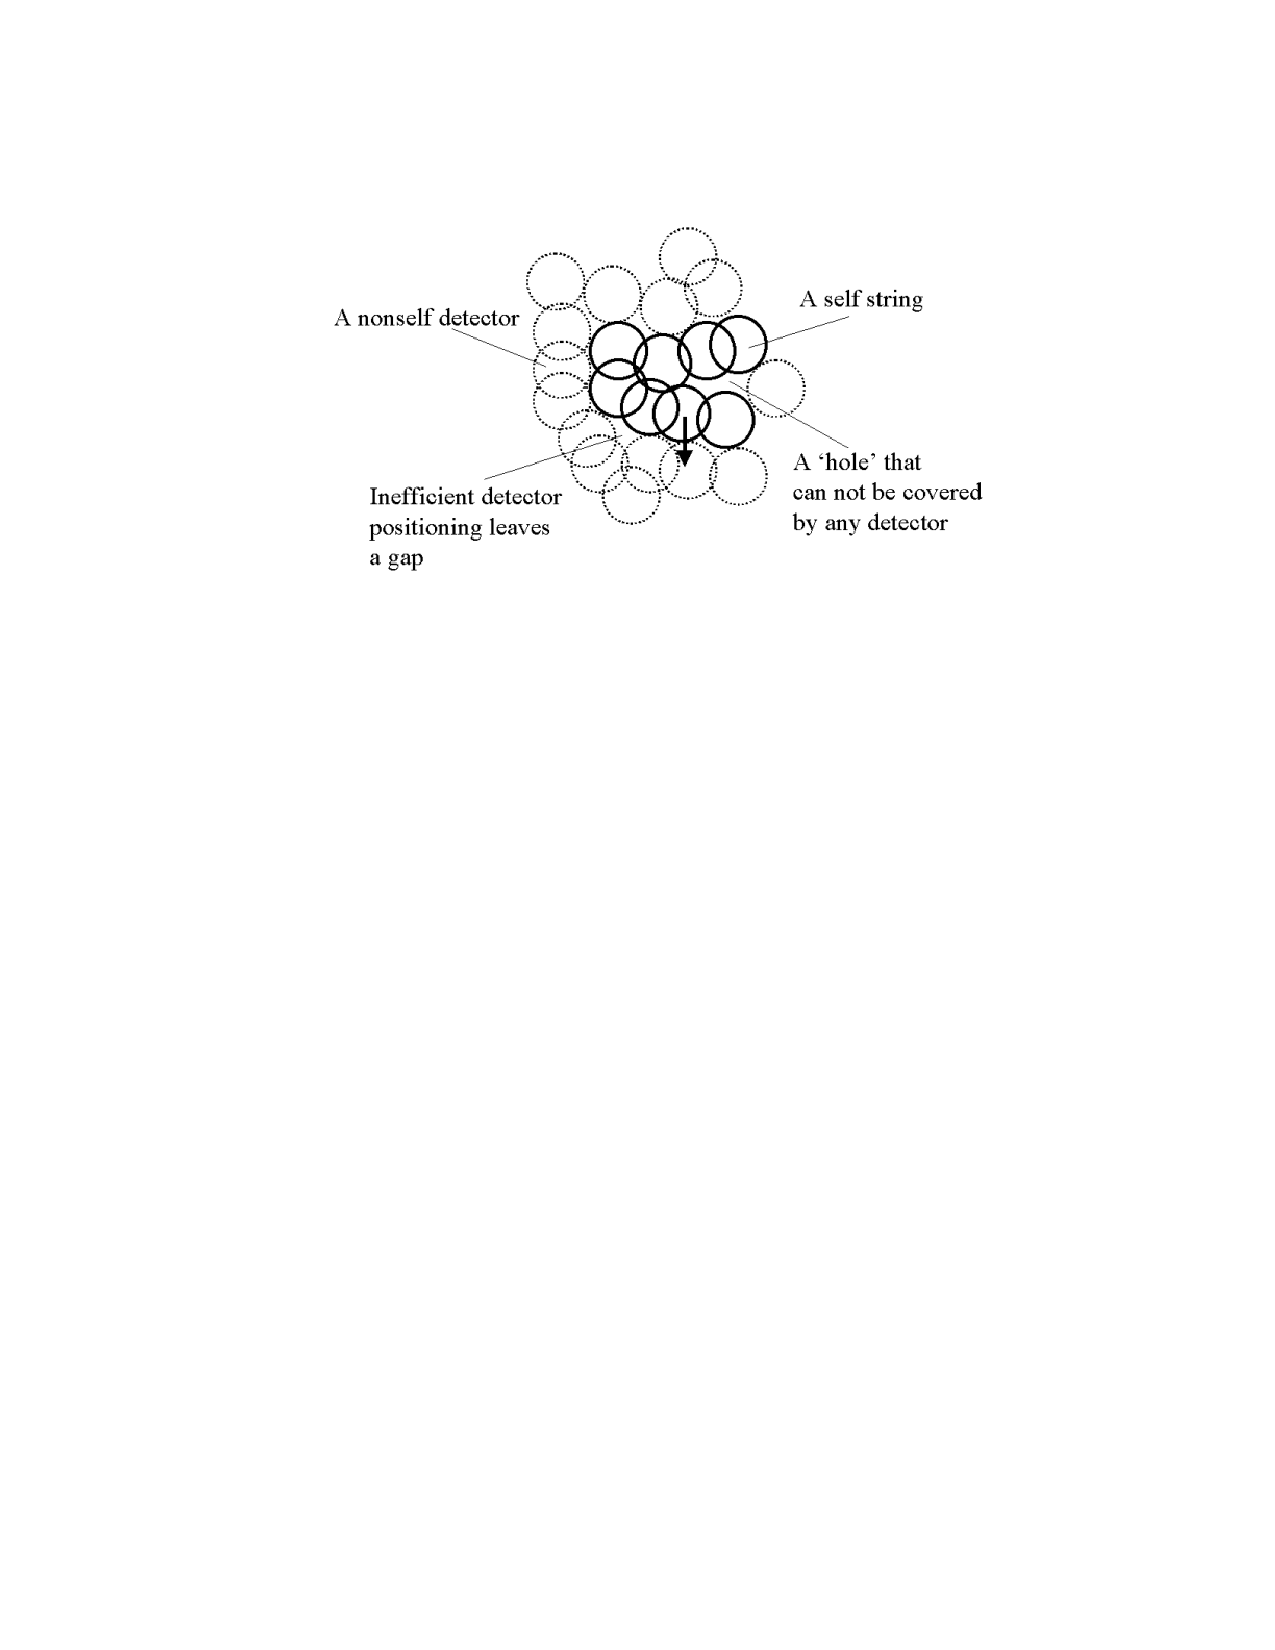
\includegraphics[width=3in, height=1.5in]{images/holes.pdf}
\caption{Spatial depiction of detectors and two types of areas that Negative Selection algorithm detectors typically don't cover~\cite{evalAIS:2005}}
\label{fig:hole}
\end{figure}
Holes become helpful in the event of a hacker attempting to determine the information of a protected file system by altering detectors and analyzing what actions set off the network's IDS. Since IDs are not based solely on exact matching, when an intruder attempts to gain information about the system, they might get one of three things: actual information, a hole in the self/non-self population or an entity that only partially matches something in the protected system.

\pagebreak
\subsection{Paradigm shifts in AIS}
NSAs seemed quite promising early on, but around 2002 they lost a lot of support. Attempts to reduce the computational complexity of generating detectors were made, but even with these additions, it was discovered that the intrusion detection rate was less than 16\%. Also, based on just 20 minutes of data input to the negative selection IDS, to attain detection rates of 80\%, the system would need approximately 1,429 years to generate an appropriate detector. 

Around 2002, Aicklein and Cayzer introduced the topic of Danger Theory, which was based on the ability to discriminate between varying contexts. From this, a specialized API called \textit{libtissue} was developed grounded in specific immunological principles. These included: the ability for a system to have various categories of cell types, said cells should have the ability to communicate amongst one another, cell types should be segregated (compartmentalized) based on maturation and allowed to communicate once they both reach a particular state, and, finally, cells should be allowed to be variable yet some type of genome-like object should be incorporated to remember previous threats (i.e. some amount of an object similar to signature databases).  The \textit{libtissue} API was developed to test and run varying immune-inspired algorithms. The Dendritic Cell Algorithm, described in the following section, is one such approach
\cite{greensmith_thesis:2007}.

\section{Dendritic Cell Algorithm}
\label{sec:Dendritic Cell Algorithm}
\subsection{Overview}
The Dendritic Cell Algorithm (DCA), an AIS inspired algorithm, attempts to detect intrusions by mimicking dendritic cells (DC), which are the first line of defense in the natural immune system. The DCA uses a population of dendritic cell objects. Each dendritic cell begins in an immature state and collects a library of `antigens' that constantly enter the system at varying rates. Alongside this process, these DC objects also analyze constant input signals to the system. Each process ID (PID) in a system is defined as an antigen type, and every time a process sends an instruction to the operating system's kernel, an antigen with that PID's number is created and put into the system's current antigen vector to be collected by the dendritic cells. 

Signals come in four types, with each signal type being a unique mapping of raw data to a particular format. The dendritic cells combine these four signals to determine two things. First, when to stop sampling signals, and second, what context the antigens collected by a DC will be saved as in the `lymph node's' antigen library. When a DC has received a sufficient amount of signals (this limit will be described in Section~\ref{sec:outputSignals}), based on the amount of each signal type received, the immature DC becomes either semi-mature or fully-mature. The process and equations that determine which maturity state a DC changes to will be depicted in Sections~\ref{sec:outputSignals} and~\ref{sec:anomalyCoefficient}. Finally, at certain intervals, the algorithm is stopped and analysis is performed on the aggregate list of stored antigens to determine how anomalous each process is at the current moment.

\subsection{Input Signals}
The dendritic cell algorithm maps the system's raw data input into four signal types. Each signal's exact computational equivalent will be described in Section~\ref{sec:expSetup}. The first signal, Pathogen Associated Molecular Pattern (PAMP), biologically speaking, are produced by microorganisms, but not by the host, and correspond to invasions.  Danger signals in the NIS represent stress and unexpected cell death. The third signal type, safe signals, are the signals received when a cell dies at its expected time. The final signal type, not always used, is inflammation. From a biological perspective, in the presence of an intrusion, the NIS would want to prepare the supposedly infected area for quick repair, hence it allocates more resources to said area. In terms of the DCA, inflammation doubles the strength of all signals to speed up the detection process. 

\subsection{Signal Processing and Output Signals}
\label{sec:outputSignals}
Throughout its life, a DC samples all input signals once every second and uses the categorized signal types in three different weighted sum equations to derive three different output signals. 

In the immune system, certain DCs receive more or less signal input than other DCs because distribution is not perfectly equal everywhere; to model this, DCs in the DCA are given a randomized value, termed migration threshold, which determines the amount of time they spend sampling signals and antigens. 
If the first output signal, the co-stimulatory (CSM) signal at any point is greater than the migration threshold, the immature DC ceases sampling signals and antigen, changes into either a semi-mature or fully-mature dendritic cell and then presents its stored antigens and calculated output signals to the antigen storage library (a log file in this case). The DC is then reset and put back into the population to maintain a constant population size.  

CSM's calculation is described in Equation~\ref{eq:csm} and includes $W_{1}$ a weight defined by the user to affect how long DCs collect signals for. Weights are applied to the sum of the PAMP signals ($P_i$) collected by an immature DC, and added to the sum of both the DC's Danger ($D_i$) and Safe signals ($S_i$). Finally the inflammation value I (either 1 or 0) is incorporated if inflammation is being used in the implementation of the DCA.
\begin{equation}
\label{eq:csm}
\big(W_{1}\sum_i^n  P_{i} + \frac{W_{2}}{2}\sum_i^n  D_{i} + 1.5W_{1}\sum_i^n  S_{i}\big)* \big(1+I\big) 
\end{equation}
The next type of calculated output signal is the semi-mature output. The function for deriving this value is the sum of all safe signal inputs that a DC has received. This output is compared to the third output signal type, the fully-mature output signal, to determine a DC's context value. This function also uses a user-defined weight ($W_{2}$) and is almost identical to Equation~\ref{eq:csm} except that the summation of its safe signals is negated so it can have a diminishing effect on both PAMP and the danger signals. 

Once a DC's CSM surpasses its migration threshold, if the fully-mature output is greater than the semi-mature output, then the DC is given a context value of 1, and it considers all the antigens it has collected as being anomalous. If the DC's semi-mature output is greater than its fully-mature output, the DC's context value is 0 and the DC considers all of its antigen to have been collected during a period of overall normalcy.

Due to variance in individual DC migration thresholds, a system call may be viewed as anomalous by some DCs, yet seen as normal by others. This is because a DC's final maturity state is based on the overall context that it experienced over the course of its existence. 
After this process, the matured DC logs each antigen bound with its context value to a log file, resets itself to a data-less immature DC and is returned to the population.

\subsection{Determining anomaly coefficients}
\label{sec:anomalyCoefficient}
For the system to determine how anomalous a process or data item was at a particular iteration, the DCA, analyzes each~\textbf{antigen type} from information written to a log by DCs. This value of abnormality is calculated by finding the mean context value for all antigens with the same PID. This is termed as an antigen type's Mature Context Antigen Value (MCAV) and is compared against a user defined MCAV threshold. If a process' MCAV equals or surpasses this threshold, the process is considered to be anomalous.

Robert Oates made slight improvements on process to reduce computational complexity. Before, at each iteration, three signals (change in CSM, semi-mature and fully-mature) would have to be computed for the overall population, these and three signals were then added to each individual DC. Oates suggested applying an instantaneous change between the mature and semi-mature signal outputs to give each DC an anomaly context value at all times. This newer anomaly coefficient, k, is calculated as following: \textsf{k = matureOutput - semiMatureOutput}. 

With this change, a new metric, $K_\alpha$ (where $\alpha$ stands for antigen type) was used for representing how anomalous an antigen type was. A process' $K_\alpha$ was then calculated by averaging all the anomaly coefficients (k) that were spawned from the same PID~\cite{signalCalculationImprovements:2008}.
As Section~\ref{sec:stats} will show, this revised approach to calculating the abnormality of an antigen type improve the results for analysis in a proposed real-time online DCA~\cite{guSeg:2011}.

\section{DCA Applied to Port Scan}
\label{sec:DCA Applied to Port Scan}
\subsection{Overview}
Determining the running processes of a device or network is useful information to hackers. A way to gather such information is by finding out which ports in a system are ``listening and accepting connections'' \cite{greensmith_thesis:2007}; this is what port scanning attempts to do. A type of port scan called SYN scanning accomplishes this by creating what is known as `half open connections' in order to be less detectable. A major portion of SYN scan processing consumption is in generating, sending and receiving TCP reset packets (RST). The attacker sends a synchronize (SYN) packet, if the port sends a synchronize acknowledge packet (SYN-ACK), this port is open for a connection. Immediately, the attacker sends back an RST to close the connection before full contact is made so its IP is not logged. This type of real-world attack was a great test for determining the DCA's aptitude in detecting intrusions and in particular, differentiating between an anomaly or normal activity during malicious attacks. The anomalous processes to be detected as a SYN scan in this experiment were an Nmap process (a widely used scanning tool) and a pts process, which was the ssh process Nmap was run from~\cite{greensmith_thesis:2007}.
\subsection{Experimental Setup}
\label{sec:expSetup}
Two data sets were used to experiment with the DCA's ability to detecting SYN scans~\cite{greensmith_thesis:2007}. The first consisted of a SYN scan occurring alongside basic shell processes, termed passive normal (PN). One of the many shell processes that this data \textit{did} include was a Firefox process running, but this was not through the ssh daemon. The second data set, active normal (AN) was the same as the PN set, but it included a normal process which in this case was a Firefox Browser, but this \textit{was} running through the same ssh daemon as the SYN scan. This is important because SYN scan attacks are performed remotely. 
A total of seven signal categories were used in this implementation of the DCA applied to detecting SYN scans, obtained through three unique signal collection scripts; these are described below.
\paragraph{Proc file system}
The first four signal types were collected using Unix's proc filesystem (procfs), which essentially tells a user about a system's process information. 
The first, labled PAMP-1, was defined as the number of destination unreachable (DU) messages per second. These particular DUs were due to a scan attempting to find open ports. High amounts of this signal are indicative of the initial stages of a SYN scan. 

The next signal type used by procfs was a danger signal, termed DS-1. The total number of network packets being sent from the victim host at any time is the value given to DS-1. 

Procfs is also the system that generates the first type of Safe Signal (SS-1). SS-1 is calculated by taking the rate of change of DS-1. Large absolute values of this signal inform the DCA that an anomaly is present in the case of SYN scans. 
This is because the attacker generates many raw packets and suddenly sends them to various ports to determine what is and is not open. 

The final type of signal that procfs generates is inflammation. This signal is either 1 or 0 and it informs the DCA if a remote root login is present or not. 
Inflammation cannot affect the input signal to immature DCs, but if a remote root login is present, inflammation exists and the value of any signals output by both mature and semi-mature DCs are doubled.
\paragraph{Tcpstat}
The statistics for network interfaces in Greensmith's application of DCA for detecting SYN scans are determined by a tool called tcpstat. This tool obtained information such as: average packet size, total number of packets, and the number of packets being processed. One other statistic this resources gathers is the standard deviation of packet size, which is particularly important to the safe signal used for this experiment.
Tcpstat computes the ratio of TCP packets to all packets and is another form of danger signal (DS-2 in this experiment). The reason DS-2 is included is that during a SYN scan, a large amount of the traffic consists of very small TCP packets.
The other signal type that tcpstat generates is a safe signal (SS-2). The structure of SS-2 is determined by the average size of all network packets at any given time. The reasoning behind this is, at some point during a SYN scan, the average packet will be small because a large ratio of packets being sent are 40~bytes.
\paragraph{Custom Packet Sniffer}
The final signal, PAMP-2, used a custom packet sniffer to find the number of RST packets sent by the victim host and sent by the SYN scanner at any time. 
During SYN scans, for each port, an RST packet will be generated on either side regardless of the port's exploitability. Thus, a large change in amount of RST packet exchange is a strong indicator of SYN scan.

\begin{figure}
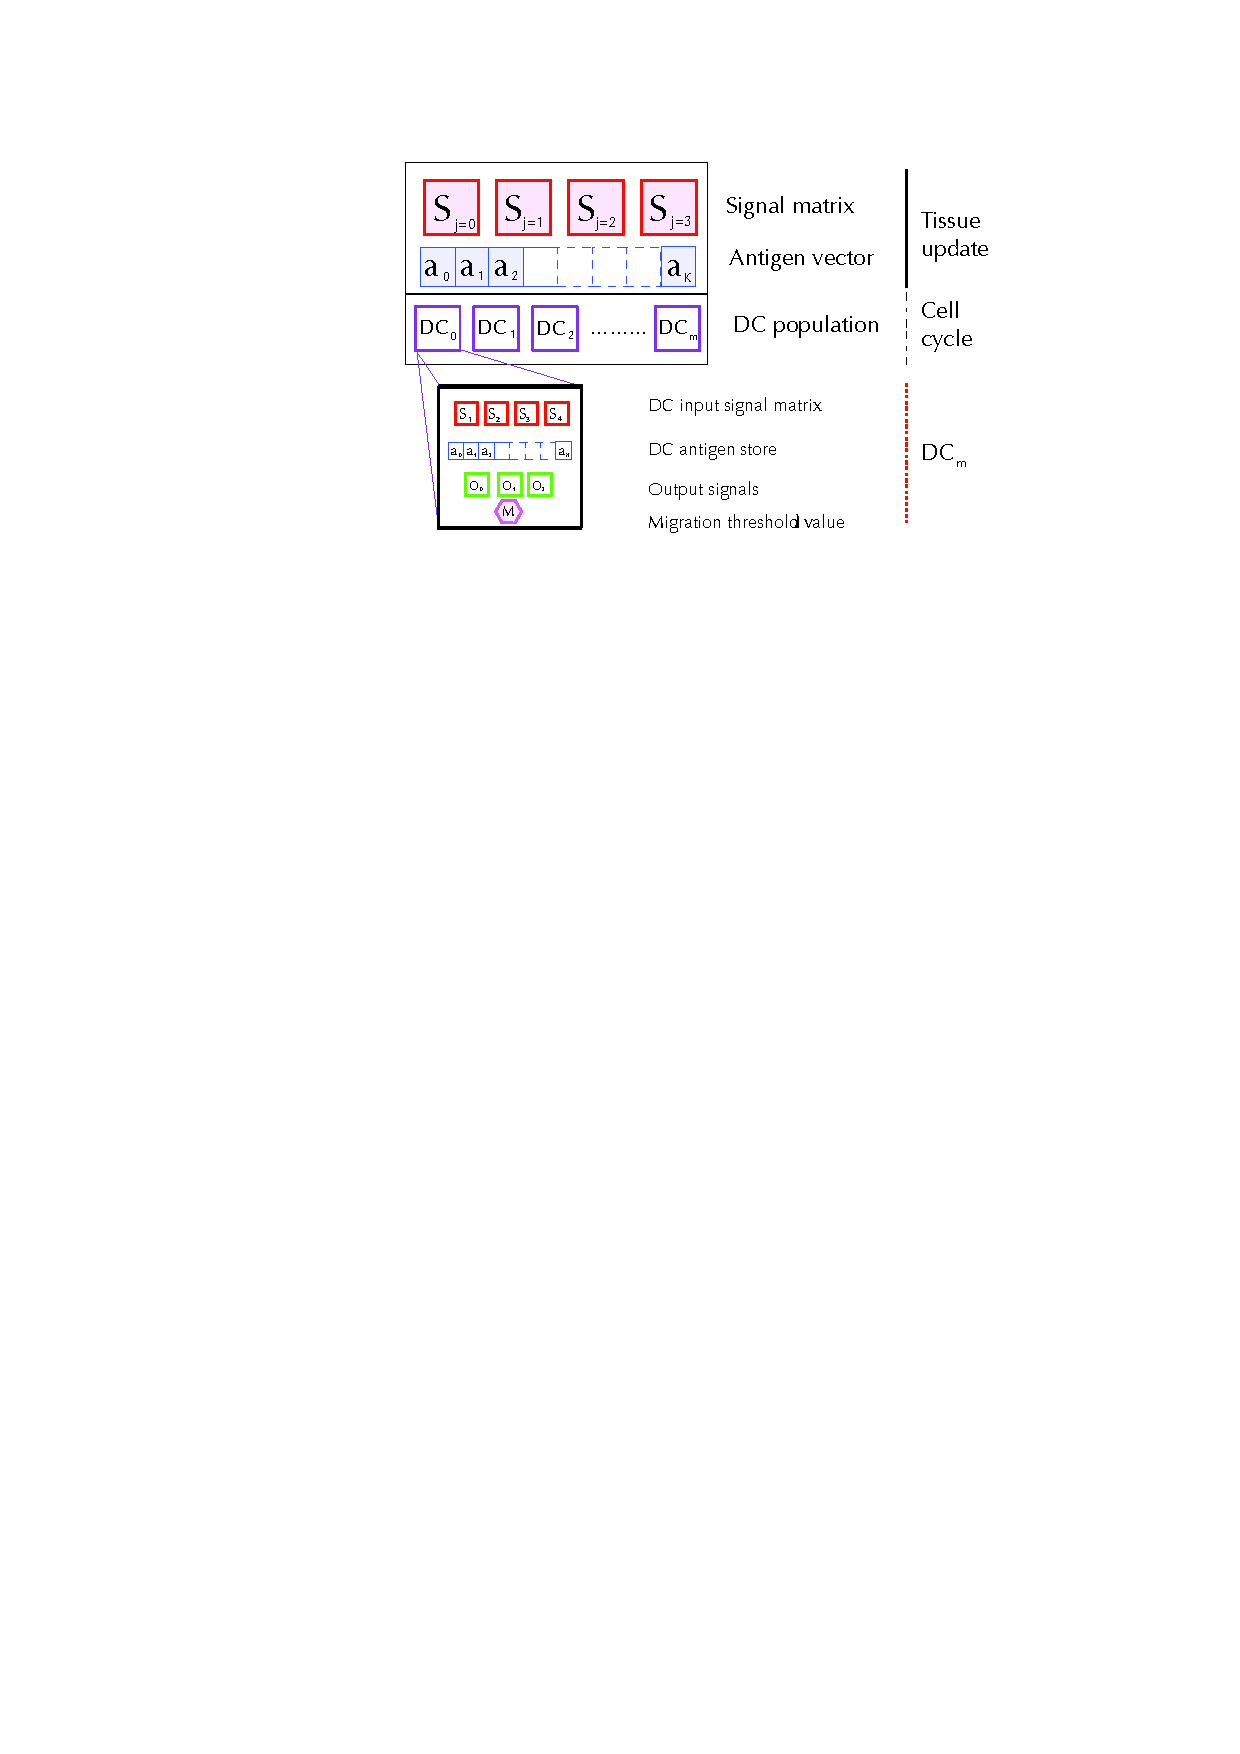
\includegraphics[width = 2.8in, height = 1.5in]{images/dcObject.pdf}
\caption{Tissue server contents illustrating makeup of a Dendritic Cell object~\cite{greensmith_thesis:2007}}
\label{fig:dcObject}
\end{figure}

\subsection{Libtissue}
The entire experiment was conducted using \textsc{libtissue}, the API mentioned previously for using real world data as a test case for various immune based algorithms. It uses a socket-based communication system using the TCP protocol to allow tissue clients and servers to talk. The tissue client is responsible for collecting both antigen and signal inputs whereas the tissue server processes input signals with a tissue update and cell cycle process. Once every second the cell cycle occurs and every immature DC is updated by allowing to receive new signals and antigens, then migrated based on its calculated CSM to write their antigen and context values to a log file for later processing. The tissue cycle involves a continual process of signal input and receives antigens only when they are newly spawned. A depiction of the tissue server and a DC object is shown in Figure~\ref{fig:dcObject}. This process continues until analysis of the antigens contained in the log file is desired. The results are discussed in the following section since Greensmith studied both the standard DCA and an added application, segmentation, on the same data-sets.

\section{Segmentation Applied to DCA}
\label{sec:Segmentation Applied to DCA}
\subsection{Setup and Segmentation Approaches}
Segmentation's main goal was to make sure that anomalies aren't missed in the intrusion detection process. If analysis is held off till the end of a run, the averaged K value for said process could end up being below the threshold needed to classify something as an anomaly thus flying under the radar. Its other goal was to possibly allow the DCA to be a real-time online intrusion detection system.

This experiment involved aggregating data so the difference between the standard DCA and addition of one of two segmentation approaches (explained in the following paragraphs) could be studied in a static environment. Data collection was ran for 6000 seconds to document both a passive normal and active normal (both described in Section~\ref{sec:expSetup}) data-set. Antigen types were stored in vector form consisting of: a PID, an amount of abnormality (K) and the number of antigens of that type presented by matured DCs. Only antigens spawned from processes running through the ssh daemon were monitored, whereas signals were taken from all traffic on the system~\cite{greensmith_thesis:2007}.

In time-based segmentation (TBS), analysis of each antigen type was performed intermittently based on a fixed time period. In Greensmith's application of TBS, four runs were made, where the total antigen library was analyzed for anomalies in intervals (segment sizes) of 1, 10, 100 and 1000 seconds~\cite{guSeg:2011}. The Firefox process running in the ssh daemon was found to be normal before the SYN scan began, but during the scan, both nmap and Firefox were determined as anomalous. Much of this has to do with the overall structure of the DCA. It determines what processes are an anomaly based on the context in which its antigens were sampled. This shows that the DCA is good at determining when and from which ssh connection an anomaly occurred. But the DCA cannot necessarily differentiate between the processes spawned from said ssh connection if they are running simultaneously~\cite{greensmith_thesis:2007}. 

Antigen-based segmentation (ABS) involved analyzing processes for abnormality after a certain amount (determined by segment size) of system calls. The concept behind varying segment size in ABS, is that segment size \textit{z}, must remain large enough so that everything isn't detected as an anomaly, but not too large that sensitivity is lost. ABS, similar to TBS, also considered the ssh daemon spawned Firefox process to be anomalous but only when the SYN scan was running~\cite{greensmith_thesis:2007}.

\subsection{Null hypotheses}
Using four null hypotheses (only three of which will be explored in this article), this experiment determined statistical significance of the differences between the non-segmented and segmented DCA, and the differences between TBS and ABS.
The first two hypotheses tested the algorithm's overall performance for offline analysis, whereas the third hypothesis was focused on evaluating the DCA's performance at each segment, or step by step as would be needed in an online real-time evaluation. 
Null hypothesis $\textbf{H}_{5.1}$ stated that overall, segmenting the DCA's output will not affect the anomaly metrics (both MCAV and $K_{\alpha}$). Null hypothesis $\textbf{H}_{5.2}$ assumes that the overall MCAV or $K_{\alpha}$ of an antigen type would not be significantly different if the segment size was altered. 
Finally, null hypothesis $\textbf{H}_{5.3}$ assumed that no difference in detection accuracy would be expected between the standard non-segmented DCA and the DCA with segmentation. When the MCAV or $K_\alpha$ of a normal process is less than the user defined anomaly threshold, a true negative (TN) has occurred. A true positive (TP) is defined as the MCAV or $K_\alpha$ of an anomalous process surpassing the same user defined anomaly threshold. To determine detection accuracy at any given point, the number of TPs and TNs are added, then divided by the total number of PIDs.
After analyses were completed on all non-segmented and segmented runs, Mann-Whitney tests were conducted in an attempt to reject these null hypotheses~\cite{guSeg:2011}.

\subsection{Statistical Tests}
\label{sec:stats}
Statistically significant different $K_\alpha$ values were found for true anomalies (Nmap and pstat) when comparing the non-segmented DCA to the DCA with ABS. Statistically significant differences were also reported for detection of normal processes when comparing time based segmentation versus the non-segmented DCA. These results rejected the first null hypothesis $\textbf{H}_{5.1}$ and proved that segmentation had a positive impact on the DCA's ability to detect anomalies and normal activity. Statistically significant differences were also seen between differing segment sizes in the analysis. Thus $\textbf{H}_{5.2}$ was rejected and it was shown that segment size had an impact on anomaly detection. Finally, null hypothesis $\textbf{H}_{5.3}$ was rejected but only with respect to $K_\alpha$. This meant that better detection accuracy was achieved through segmentation than with the standard non-segmented DCA when using the anomaly metric $K_\alpha$. These results showed that segmentation could be used as an online component for the DCA. The speculated reason for $K_\alpha$ providing an increase in accuracy with segmentation (where MCAV couldn't) was that $K_\alpha$ was a real valued number as opposed to a 1 or 0, and was thus a more accurate depiction of a DCA's overall anomaly context value.

\subsection{Results and Future Work}
The results from the statistical analysis verified that segmentation could improve the identification of normal and anomalous processes, but this improvement was constrained by segment size and whether antigen-based segmentation or time-based segmentation was used. Both types of segmentation were shown to improve detection accuracy when using the $K_\alpha$ anomaly metric. Also, the results determined that segmentation could, in parallel, provide continuous and periodic analysis of signal outputs. Variation in segment size was shown to improve the detection performance of the DCA as well. Analysis of sensitivity could be used in the future to find optimal segment size. Using this, segmentation size could be dynamic in order to further improve the results of the DCA
\cite{guSeg:2011}.
The Dendritic Cell Algorithm functioned well in detecting anomalies, but it can produce strong false positives during the time of attack on processes that were created from the same ssh daemon spawned attack~\cite{greensmith_thesis:2007}.

\section{Conclusion}
\label{sec:Conclusion}
The field of intrusion detection is constantly becoming more complex and various traditional techniques are not as viable as they once used to be. There are numerous categories that intrusion detection systems are comprised of and each approach in these disparate categories have their individual strengths and weaknesses. 

New approaches such as the application of artificial immune systems are promising for intrusion detection, but the field is still young and many of its algorithms are composed of biologically naive structures that date back to the 50s~\cite{greensmith_thesis:2007}.

Recently, new immune inspired techniques such as the dendritic cell algorithm have been developed in an attempt to overcome these obstacles in intrusion detection. This algorithm has been proven to have validity in the field of intrusion detection. Also, the implementation of dynamic segmentation has been postulated to significantly improved this algorithm's results. But more improvements need to be made before the dendritic cell algorithm is fully feasible for real-time applications to everyday computing.

\nocite{*}
%^this is a very important addition so that
%references will be included property

\bibliography{Bibliography}
\bibliographystyle{abbrv}
\end{document}